\chapter{Revisão Teórica}
\section{Introdução a Lógica Modal}
\label{sec:l_gica_modal}
Neste capítulo, introduziremos a lógica modal através do sistema $S5$. Este
sistema, apesar de ser um dos mais simples possíveis, possui algumas das
principais características do sistema de lógica modal, e essas serão ilustradas
a partir dele. 

O sistema $S5$ é determinado semanticamente por uma avaliação de necessidade e
possibilidade.
Isto é, em resumo %forçado
, a base da estrutura do pensamento modal que data desde o filósofo Leibniz: uma
proposição é \textit{necessária} se ocorre em todos os possíveis mundos 
e \textit{possível} se ocorre em algum mundo~\cite{chellas:modal_logic}.
A ideia é que coisas %revise
diferentes podem ser verdadeiras em mundos diferentes, mas qualquer que ocorra
em todos os possíveis mundos é necessário, enquanto o que ocorre em pelo menos
um mundo é possível.

%As proposições são da forma $\Box A$
%$\Diamond A$

Uma sentença da forma $\Box A$ --- \textit{necessariamente} $A$ --- é verdadeira se,
e somente se, $A$ é uma proposição verdadeira em todos os possíveis mundos; já
uma sentença da forma $\Diamond A$ --- \textit{possivelmente} $A$ --- é verdadeira
no caso em que $A$ é uma proposição verdadeira em algum possível mundo.

Uma ilustração válida é uma coleção de possíveis mundos, incluindo nosso
próprio, o mundo real, onde sentenças da linguagem são possivelmente verdadeiras
ou falsas. O propósito principal da lógica modal é modelar isto, e isto é feito
listando uma sequência possivelmente infinita de conjuntos de possíveis mundos,
\begin{equation}
    P_0,\ P_1,\ P_2,\ldots
\end{equation}

A intuição por trás deste modelo é que, para cada número natural $n$, o conjunto
$P_n$ contém somente os possíveis mundos onde a sentença $\mathbb{P}_n$ é
verdadeira. Em outras palavras, a sequência 
$P_0,\ P_1,\ P_2,\ldots$
ilustra as sentenças at\^omicas estipulando em quais possíveis mundos elas
ocorrem, e.g onde são verdadeiras,
(e, por omissão, em quais mundos elas são falsas):
\begin{equation}
    \mathbb{P}_n\ is\ true\ at\ a\ possible\ world\ \alpha\ if\ and\ only\ if\
    \alpha \in P_n 
\end{equation}

Um modelo no sistema $S5$ é, portanto, uma tupla:
<$W$,~$P$>
onde $W$ é um conjunto de possíveis mundos e $P$ uma abreviação para a sequência
infinita 
$P_0,\ P_1,\ P_2,\ldots$
de subconjuntos de $W$.
Note que $W$ pode conter mundos que não estão presentes em nenhum dos conjuntos
$P_n$; de fato, qualquer um desses conjuntos pode ser vazio.

Definimos o valor da sentença (verdadeiro ou falso) de acordo com sua forma e em
termos de um possível mundo em um modelo.
Usamos a notação:
\begin{equation}
    \label{modal:truth}
    \models ^{\mathcal{M}}_{\alpha} A 
\end{equation}
onde $A$ é uma sentença e $\alpha$ é um possível mundo em um modelo
$\mathcal{M}=<W,P>$.
A lei~\ref{modal:truth} é um resumo para: $A\ is\ true\ at\ \alpha\ in\
\mathcal{M}$.

As condições de verdade estão expressadas na Tabela~\ref{table:truth}.

\begin{center}
    \begin{table}[h!]
\label{table:truth}
    \caption{Truth conditions}

    \begin{tabular}{ll}

        \vspace{2mm}
        (1) & $\models ^{\mathcal{M}}_{\alpha} \mathbb{P}_n$ se e somente se $\alpha \in
        P_n$ com $n=0,1,2,\ldots$\\
        \vspace{2mm}
        (2)  & $\models ^{\mathcal{M}}_{\alpha} $\\
        \vspace{2mm}
        (3)  & $Not\ \models ^{\mathcal{M}}_{\alpha} $\\
        \vspace{2mm}
        (4)  & $\models ^{\mathcal{M}}_{\alpha} \neg A$ se e somente se $not\
        \models ^{\mathcal{M}}_{\alpha} A$\\
        \vspace{2mm}
        (5)  & $\models ^{\mathcal{M}}_{\alpha} $\\
        \vspace{2mm}
        (6)  & $\models ^{\mathcal{M}}_{\alpha} $\\
        \vspace{2mm}
        (7)  & $\models ^{\mathcal{M}}_{\alpha} $\\
        \vspace{2mm}
        (8)  & $\models ^{\mathcal{M}}_{\alpha} $\\
        \vspace{2mm}
        (9)  & $\models ^{\mathcal{M}}_{\alpha} \Box A $\\
        \vspace{2mm}
        (10) & $\models ^{\mathcal{M}}_{\alpha} \Diamond A $\\

    \end{tabular}
\end{table}
\end{center}

Alguns esclarecimentos sobre essas definições podem ser úteis:
\begin{itemize}
    \item A cláusula (1) reflete a premissa sobre os conjuntos $P_0, P_1, P_2,
        \ldots$ em um modelo: uma sentença at\^omica $\mathbb{P}_n$ é verdadeira
        em um possível mundo $\alpha$ somente no caso em que $\alpha$ é um
        elemento do conjunto $P_n$.
    \item De acordo com a cláusula (2), a constante verdadeira $\top$ é sempre
        válida em $\alpha$.
    \item Por (3), a constante falsa $\bot$ é sempre falsa em $\alpha$.
    \item A cláusula (4) afirma que a negação $\neg A$ é verdadeira em $\alpha$
        se, e somente se, sua negação $A$ é falsa em $\alpha$.
    \item A afirmação da cláusula (5) diz que uma conjunção $A \wedge B$ é
        verdadeira em $\alpha$ somente no caso em que ambas sentenças, $A$ e
        $B$ o são.
    \item Já de acordo com a cláusula (6), uma disjunção $A \vee B$ é verdadeira
        em $\alpha$ quando pelo menos uma das sentençãos, $A$ ou $B$ o é.
    \item A inteção com a cláusula (7) é compreender que uma implicação $A \rightarrow
        B$ é verdadeira em $\alpha$ desde que nunca ocorra que a sentença antecedente,
        $A$, seja verdadeira ao mesmo tempo em que a consequente, $B$, seja
        falsa.
    \item Similarmente, na cláusula (8) a intenção se repete de ambos os lados,
        ou seja, a condição $A \leftrightarrow B$ é verdadeira quando ambas
        sentenças, $A$ e $B$, são verdadeiras, ou ambas são falsas.
    \item A cláusua (9) formula a interpretação leibniziana de necessidade:
        $\Box A$
    \item Finalmente, de acordo com a cláusula (10), $\Diamond A$
\end{itemize}

Uma sentença verdadeira em cada mundo possível de todo modelo é chamada
\textit{válida}. Usamos o símbolo $\models$ novamente, mas desta vez sem as
marcações superior e inferior (para enfatizar que a sentença é válida, sem
importar o mundo ou o modelo), e escrevemos $\models A$ quando $A$ é uma
sentença válida.
Mais formalmente, então, definimos a validade de uma sentença da seguinte forma:

\begin{equation}
    \models A\ se,\ e\ somente\ se,\ para\ todo\ modelo\ \mathcal{M}\ e\ para\ 
    qualquer\ mundo\ \alpha\ em\ \mathcal{M},\ temos\ que\ \models ^{\mathcal{M}}_\alpha 
\end{equation}


%% KEEP ON BABY

\begin{figure}
\label{figure:mundos_simples}
\begin{center}
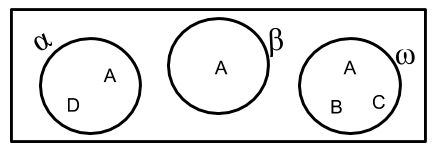
\includegraphics[scale=0.8]{imagens/ex_modal_simples.png}
\caption{Exemplo lógica modal}
\end{center}
\end{figure}

%??
\section{Preliminares lógicas}
\subsection{Sintaxe}

Esta seção é dedicada a trazer o básico dos conceitos de sintaxe da linguagem da
lógica modal. As definições formais apresentadas podem ser úteis ao
entendimento.

\textbf{Sentenças.} A linguagem é baseada em um conjunto enumerável de sentenças
\textit{at\^omicas}: 
\begin{equation}
    \mathbb{P}_0, \mathbb{P}_1, \mathbb{P}_2, \ldots 
\end{equation}
Estas são as sentenças mais simples possívels.

As \textit{sentenças moleculares} (não-at\^omicas) são formadas por meio das nove
\textit{operações sintáticas}, ou \textit{operadores lógicos}:
\begin{equation}
   \top, \bot, \neg, \wedge, \vee, \rightarrow, \leftrightarrow, \Box, \Diamond
\end{equation}

Como mencionado na seção anterior, $\top$ e $\bot$ são operadores de aridade
zero, ou constantes; $\neg$, $\Box$ e $\Diamond$ são operadores de aridade um; e
$\wedge$, $\vee$, $\rightarrow$ e $\leftrightarrow$ são operadores de aridade
dois.

O conjunto de sentenças pode, então, ser definido formalmente como mostrado na
Tabela~\ref{table:sentences}.

\begin{center}
    \begin{table}[h!]
\label{table:sentences}
    \caption{Truth conditions}

    \begin{tabular}{ll}
        \vspace{2mm}
        (1) & a \\
        \vspace{2mm}
        (2)  & a \\
        \vspace{2mm}
        (3)  & a \\
        \vspace{2mm}
        (4)  &a \\
        \vspace{2mm}
        (5)  & a \\
        \vspace{2mm}
        (6)  &a \\
        \vspace{2mm}
        (7)  &a \\
        \vspace{2mm}
        (8)  &a \\
        \vspace{2mm}
        (9)  &a \\
        \vspace{2mm}
        (10) &a
    \end{tabular}
\end{table}
\end{center}

As sentenças at\^omicas são todas distintas entre si, e a intenção é que sentenças
de formas diferentes também sejam distintas, como, por exemplo, nenhuma sentença
condicional é uma necessidade. Isto é garantido pela suposição de que o alcance
dos operadores sintáticos é disjunto dois a dois e ainda, disjunto do conjunto
de sentenças at\^omicas.
A falta de ambiguidade das sentenças é garantida pela suposição de que as
operações são todas \textit{um-pra-um}, ou seja, duas condicionais são, por
exemplo, iguais se, e somente se, ambos antecedentes e consequentes o são.
Também é válido lembrar que o conjunto de sentenças é enumerável.

\textbf{Convenções.} É importante definir algumas convenções para minimizar 
dúvidas que poderiam surgir em algumas expressões.
Expressões da forma $A_1 \wedge \ldots \wedge A_n$ e $A_1 \vee \ldots \vee A_n$
representam conjunções e disjunções arbitrárias mas não especificadas das
sentenças $A_1,\ldots,A_n$. O objetivo é clarificar que tanto $\wedge$ como
$\vee$ obedecem as regras de associatividade lógica. 

\subsubsection{Fórmulas}
Uma \textit{fórmula} é qualquer sequência finita de símbolos lógicos. 

\begin{definition}[Fórmula bem-formada (FBF)]
    A lingagem lógica proposicional, denotada por $L_p$, é equivalente ao seu
    conjunto de fórmulas bem-formadas, denotado por $FBF_{L_P}$, que é definito
    recursivamente como segue:
    \begin{itemize}
        \item se $p \in P$, então $p \in FBF_{L_P}$
            \item se $\phi \in FBF_{L_P}$ e $\varphi \in FBF_{L_P}$, então: $\neg
                \phi,\ (\wedge), (\vee), (\rightarrow), (\leftrightarrow) \in FBF_{L_P}$, 
            
    \end{itemize}
\end{definition}

\subsection{Semântica}

\section{Modelos padrões para a lógica modal}
\label{sec:modelos_padroes}

A ideia geral dada na seção~\ref{sec:l_gica_modal} é bastante simples, sendo
modelada basicamente em termos de uma coleção de possíveis mundos junto com uma
atribuição de valores booleanos, em cada mundo, a cada uma das sentenças
at\^omicas. Vimos que isso dá uma noção de validade um tanto restrita.
Nesta seção, iremos estender a definição leibniziana de necessidade e
possibilidade introduzindo o conceito de relações. O resultado é uma noção de
validade muito mais flexível.

Um modelo padrão será estruturado da seguinte forma:
\begin{equation}
    \label{eq:mod_padrao}
    \mathcal{M} =\ <W,R,P>
\end{equation}
onde $W$ representa o conjunto de possíveis mundos, $P$ representa a atribuição
dos subconjuntos de possíveis mundos a cada sentença at\^omica e o novo elemento
$R$, é uma relação entre possíveis mundos, ou seja, $R$ é uma relação binária em
$W$ ($R \subseteq W \times W$).

Escreveremos
\begin{equation}
    \alpha R \beta
\end{equation}
para dizer que o mundo $\beta$ está relacionado com, ou é relevante para, o
mundo $\alpha$. É importante ressaltar que $R$ pode ser qualquer tipo de relação
binária em $W$, nenhuma suposição é feita sobre sua estrutura.

As condições de verdade de sentenças não-modais, dadas na
Tabela~\ref{table:truth}, permanecem inalteradas. Já as relacionadas às
sentenças modais sofre uma pequena alteração, levando em conta agora, a relação
R da seguinte forma:

    \begin{table}[h!]
\label{table:truth}
\begin{center}
    \caption{Condições de verdade: sentenças modais}
    \begin{tabular}{ll}
    Seja $\alpha$ e  \\

        \vspace{2mm}
        (1) & $\models ^{\mathcal{M}}_{\alpha} \mathbb{P}_n$ se e somente se $\alpha \in
        P_n$ com $n=0,1,2,\ldots$\\
        (2)  & $\models ^{\mathcal{M}}_{\alpha} $\\

    \end{tabular}
\end{center}
\end{table}

\begin{figure}
\label{figure:mundos_relacao}
\begin{center}
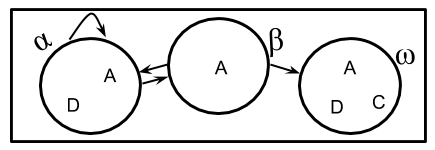
\includegraphics[scale=0.8]{imagens/ex_modal_relacao.png}
\caption{Exemplo lógica modal}
\end{center}
\end{figure}

\subsection{Lógica Multimodal}
\label{sub:lógica_multimodal}


\subsubsection{Estrutura de Kripke}

Uma das estruturas mais estudadas em lógica modal corresponde à estrutura de
Kripke. Uma estrutura de Kripke para $P$ e $A_n = \{1, \ldots, n\}$ é dada da seguinte forma:
\begin{equation}
\mathbb{M} = <W,\ R_1, \ldots,\ R_n, \pi>
\end{equation}
onde:
\begin{itemize}
    \item $W$ é um conjunto não-vazio de possíveis mundos
    \item para todo $a \in A_n, R_a \subseteq W \times W$
    \item $\pi: W \times P \longrightarrow \{Falso, Verdadeiro\}$
\end{itemize}




\section{Resolução}
\label{sec:resolucao}

\subsection{Forma Normal Negada}
\begin{definition}[Forma Normal Negada (FNN)]
    Seja $\varphi \in FBF_{L_P}$, dizemos que $\varphi$ está na Forma Normal
    Negada (FNN) se contém apenas os conectivos $\neg$, $\wedge$ e $\vee$ e o
    conectivo de negação é aplicado apenas a símbolos proposicionais.
\end{definition}

A transformação em FNN é dada pelo seguinte procedimento:
\begin{enumerate}
    \item Substitua
    \item Substitua
    \item Aplique as leis de De Morgan
    \item Elimine
\end{enumerate}

A simplificação de fórmulas aplica as seguintes regras de reescrita:
\begin{itemize}
    \item 
\end{itemize}

\subsection{Forma Normal Conjuntiva}
\begin{definition}[Forma Normal Conjuntiva (FNC)]
    Seja $\varphi \in FBF_{L_P}$, dizemos que $\varphi$ está na Forma Normal
    Conjuntiva se é uma conjunção de cláusulas.
\end{definition}

A transformação de uma fórmula $\varphi$ em uma fórmula semanticamente
equivalente, $\varphi '$, na FNC, é dada pelo seguinte procedimento:

%\subsection{Provas}
%\label{sub:provas}



\subsection{Resolução Clausal}
Resolução clausal é um procecimento refutacional: para podermos provar a
sentença $\varphi$, nós transformamos a negação de $\varphi$ na Forma Normal
Conjuntiva antes de aplicar a regra de inferência

\subsection{Tableaux}
\label{sub:tableaux}
Métodos de demonstração utilizando tableaux são frequentemente utilizados,
com sucesso, em lógica modal para prover decisões de procedimento.

O tableaux consiste em uma prova representada graficamente na forma de árvore. É
um método analítico baseado na prova por contradição.


\subsection{Tableaux Clausal}



